\documentclass[11pt, a4paper]{article}

% ─── Packages ───────────────────────────────────────────────────────────────
\usepackage[top=1.8cm, bottom=1.8cm, left=2cm, right=2cm]{geometry}
\usepackage[utf8]{inputenc}
\usepackage[T1]{fontenc}
\usepackage{lmodern}
\usepackage{microtype}
\usepackage{titlesec}
\usepackage{enumitem}
\usepackage{xcolor}
\usepackage{graphicx}
\usepackage{booktabs}
\usepackage{tabularx}
\usepackage{multicol}
\usepackage{fancyhdr}
\usepackage{tikz}
\usepackage{tcolorbox}
\usepackage{hyperref}
\usepackage{fontawesome5}
\usepackage{setspace}
\usepackage{parskip}

% ─── Colors ─────────────────────────────────────────────────────────────────
\definecolor{primary}{HTML}{0F172A}
\definecolor{accent}{HTML}{3B82F6}
\definecolor{accentdark}{HTML}{1E40AF}
\definecolor{success}{HTML}{10B981}
\definecolor{danger}{HTML}{EF4444}
\definecolor{warning}{HTML}{F59E0B}
\definecolor{muted}{HTML}{64748B}
\definecolor{lightbg}{HTML}{F1F5F9}
\definecolor{cardgray}{HTML}{F8FAFC}

% ─── Hyperref ───────────────────────────────────────────────────────────────
\hypersetup{
    colorlinks=true,
    linkcolor=accentdark,
    urlcolor=accent,
    pdfauthor={Team SecDev},
    pdftitle={SecDev -- Autonomous Security Testing Platform},
}

% ─── Section Formatting ────────────────────────────────────────────────────
\titleformat{\section}
  {\Large\bfseries\color{primary}}
  {\thesection.}{0.5em}{}[\vspace{-4pt}\textcolor{accent}{\rule{\textwidth}{1.5pt}}]

\titleformat{\subsection}
  {\large\bfseries\color{accentdark}}
  {\thesubsection}{0.5em}{}

\titleformat{\subsubsection}
  {\normalsize\bfseries\color{primary}}
  {\thesubsubsection}{0.5em}{}

\titlespacing*{\section}{0pt}{12pt}{5pt}
\titlespacing*{\subsection}{0pt}{8pt}{3pt}
\titlespacing*{\subsubsection}{0pt}{6pt}{2pt}

% ─── Header / Footer ───────────────────────────────────────────────────────
\pagestyle{fancy}
\fancyhf{}
\renewcommand{\headrulewidth}{0pt}
\fancyfoot[C]{\small\color{muted}\thepage}
\fancyhead[R]{\small\color{muted}SecDev\enspace\textbar\enspace Autonomous Security Platform}

% ─── tcolorbox styles ──────────────────────────────────────────────────────
\tcbset{
  highlight/.style={
    colback=lightbg, colframe=accent, boxrule=0.6pt,
    arc=3pt, left=8pt, right=8pt, top=6pt, bottom=6pt,
    fonttitle=\bfseries\color{white},
    coltitle=white, colbacktitle=accent,
  },
  graycard/.style={
    colback=cardgray, colframe=muted!30, boxrule=0.3pt,
    arc=3pt, left=8pt, right=8pt, top=6pt, bottom=6pt,
  }
}

% ─── Custom Commands ───────────────────────────────────────────────────────
\newcommand{\tech}[1]{\texttt{\small\color{accentdark}#1}}
\newcommand{\sevtag}[2]{%
  \tikz[baseline=(X.base)]\node[fill=#1!12, text=#1!80!black,
    rounded corners=2pt, inner sep=2pt, font=\scriptsize\bfseries](X){#2};%
}

\setlength{\parskip}{4pt plus 1pt minus 1pt}

% ═══════════════════════════════════════════════════════════════════════════
\begin{document}

% ─── PAGE 1: TITLE PAGE ────────────────────────────────────────────────────
\thispagestyle{empty}
\begin{tikzpicture}[remember picture, overlay]
  \fill[accent] (current page.north west) rectangle
    ([yshift=-5cm]current page.north east);
  \fill[accentdark, opacity=0.35]
    ([yshift=-2cm]current page.north west) --
    ([yshift=-5cm]current page.north west) --
    ([yshift=-3cm, xshift=9cm]current page.north west) -- cycle;
\end{tikzpicture}

\vspace*{0.5cm}
\begin{center}
  {\fontsize{42}{48}\selectfont\bfseries\color{white}SecDev}\\[8pt]
  {\LARGE\color{white!90}Autonomous Security Testing Platform}\\[4pt]
  {\normalsize\color{white!75}Zero-Configuration \,\textbar\, Sandbox-Isolated \,\textbar\, AI-Powered}
\end{center}

\vspace{1.8cm}

\begin{tcolorbox}[highlight, title={\faShieldAlt\enspace Hackathon Problem Statement}]
\textbf{Autonomous Security Systems} --- \textit{``Create self-learning or self-adaptive security solutions that reduce human intervention in monitoring, detection, and response.''}
\end{tcolorbox}

\vspace{0.4cm}

\begin{tcolorbox}[graycard]
\begin{spacing}{1.2}
{\normalsize
\textbf{What is SecDev?}\enspace SecDev is a platform that automatically tests web applications for security vulnerabilities. A developer simply connects their GitHub repository, and SecDev takes over --- it deploys the app in a secure, isolated sandbox, runs \textbf{6 different security scanners} plus functional, performance, and real-browser tests, and produces a detailed report with a security score out of 100 and step-by-step fix recommendations.

\vspace{4pt}
\textbf{Why does it matter?}\enspace Most developers don't have security expertise, and hiring security testers or buying commercial tools is expensive. SecDev makes enterprise-grade security testing available to \textit{everyone} --- for free, in one click, with zero setup.

\vspace{4pt}
\textbf{How is it autonomous?}\enspace The entire process --- from deploying the app, discovering every route and API endpoint, running all attacks, scoring vulnerabilities, to generating a human-readable report with AI --- happens \textit{without any human input}. The user only clicks ``Scan.''
}
\end{spacing}
\end{tcolorbox}

\vspace{0.4cm}

% Key stats strip
\begin{center}
\begin{tikzpicture}
  \foreach \icon/\val/\lbl/\xpos in {
    \faSearch/6/Security Scanners/0,
    \faCogs/7/Pipeline Steps/4.5,
    \faChartBar/5/Test Categories/9,
    \faBug/OWASP/Top-10 Coverage/13.5} {
    \node[fill=lightbg, rounded corners=4pt, minimum width=3.6cm,
          minimum height=1.6cm, inner sep=4pt] at (\xpos,0) {};
    \node[font=\Large\color{accent}] at (\xpos, 0.35) {\icon};
    \node[font=\large\bfseries\color{primary}] at (\xpos, -0.05) {\val};
    \node[font=\scriptsize\color{muted}] at (\xpos, -0.42) {\lbl};
  }
\end{tikzpicture}
\end{center}

\vspace{0.3cm}

\begin{tcolorbox}[graycard]
\small
\textbf{Complete User Flow:}\enspace
\faSignInAlt\enspace Login via GitHub OAuth
\;\faArrowRight\;\faCodeBranch\enspace Select a repository
\;\faArrowRight\;\faRocket\enspace Auto-deploy to sandbox
\;\faArrowRight\;\faPlay\enspace Run tests (one click)
\;\faArrowRight\;\faFileAlt\enspace View scored report with AI recommendations
\end{tcolorbox}

\vspace{\fill}
\begin{center}
\small\color{muted}\textit{Hackathon Project Report}
\end{center}

\newpage

% ─── PAGE 2: PROBLEM + HOW IT WORKS ────────────────────────────────────────

\section{Problem Statement \& Motivation}

Today, most web applications go live \textbf{without proper security testing}. The reasons are simple:

\begin{itemize}[leftmargin=1.4em, itemsep=4pt]
  \item \textbf{Security tools are expensive.} Commercial DAST (Dynamic Application Security Testing) tools like Burp Suite Pro or Acunetix cost \$10K--100K per year. Small teams and student projects cannot afford them.
  \item \textbf{They require expertise.} Even free tools like OWASP ZAP need manual configuration --- selecting scan policies, defining target scope, writing authentication scripts, and interpreting raw output.
  \item \textbf{Testing is slow and manual.} A typical security audit takes days to weeks. Developers ship code daily, so security reviews are always behind.
  \item \textbf{Results are hard to act on.} Most tools dump hundreds of raw findings with no prioritization or fix guidance. Developers don't know where to start.
\end{itemize}

The hackathon challenge asks for a system that \textbf{reduces human intervention} in security monitoring, detection, and response. SecDev answers this by reducing human intervention to \textbf{zero} --- the user clicks one button and receives a complete, scored, actionable security report.

\section{How SecDev Works --- The Full Pipeline}

When a user clicks ``Scan,'' SecDev runs the following steps automatically. Every step is managed by \textbf{Inngest} (a workflow engine), so if any step fails, it retries \textit{just that step} without starting over.

\subsection{Step 1: Deploy the App in a Sandbox}
SecDev clones the user's GitHub repository and deploys it inside an \textbf{E2B Firecracker microVM} --- the same isolation technology that powers AWS Lambda. Each user gets their own sandbox, completely isolated from other users and from production systems. This means tests can safely send attack payloads without any risk to real systems.

\subsection{Step 2: Auto-Discover All Routes}
SecDev scans the app's filesystem to automatically find every page route (like \texttt{/about}, \texttt{/dashboard}) and every API endpoint (like \texttt{/api/users}, \texttt{/api/auth/login}). No configuration file is needed --- it reads the folder structure (Next.js convention) and builds a complete route map.

\subsection{Step 3: Plan Tests Intelligently}
Based on the discovered routes, SecDev creates a test plan. It treats \textbf{page routes} and \textbf{API routes} differently --- API routes get injection testing, authentication bypass checks, and rate-limit tests, while page routes get browser-based UX testing, accessibility checks, and header analysis.

\subsection{Step 4: Run 6 Security Scanners in Parallel}
This is the core of SecDev. Six specialized scanners run against every discovered route:

\begin{center}
\renewcommand{\arraystretch}{1.3}
\small
\begin{tabularx}{\textwidth}{@{}l c X@{}}
\toprule
\textbf{Scanner} & \textbf{Risk Level} & \textbf{What It Does (Simple Explanation)} \\
\midrule
SQL Injection & \sevtag{danger}{CRITICAL} & Sends database attack strings (like \texttt{' OR '1'='1}) to every API. If the app leaks SQL error messages, returns HTTP 500, or takes too long (meaning a \texttt{SLEEP} command executed), a vulnerability is found. \\[2pt]
XSS & \sevtag{danger}{CRITICAL} & Sends script tags (like \texttt{<script>alert(1)</script>}) as input. If the app echoes them back unescaped in the response, attackers can inject JavaScript into other users' browsers. \\[2pt]
SSRF & \sevtag{danger}{CRITICAL} & Sends internal URLs (like \texttt{http://169.254.169.254}) as parameters. If the app fetches them and returns cloud metadata or internal files, an attacker can access private infrastructure. \\[2pt]
Auth Bypass & \sevtag{danger}{CRITICAL} & Tries accessing protected endpoints with no token, fake tokens, the JWT ``none'' algorithm trick, and default passwords like \texttt{admin:admin}. \\[2pt]
Headers & \sevtag{warning}{HIGH} & Checks if security headers (CSP, HSTS, X-Frame-Options) are present. Also detects leaked server info and insecure cookie settings. \\[2pt]
Rate Limit & \sevtag{warning}{MEDIUM} & Sends 30 rapid requests at once. If no request gets a 429 (``Too Many Requests'') response, the app lacks brute-force protection. \\
\bottomrule
\end{tabularx}
\end{center}

\subsection{Steps 5--7: Collect, Score, and Generate AI Report}
All findings are aggregated and scored using the formula: \textbf{Score = 100 $-$ (Critical $\times$ 15) $-$ (High $\times$ 8) $-$ (Medium $\times$ 3) $-$ (Low $\times$ 1)}. The scored report is then sent to \textbf{Groq/Llama 3.1} AI, which generates an executive summary, a prioritized fix list, and \texttt{curl} commands that let developers \textit{replay each attack} to verify fixes. AI is used \textit{only} in this final step --- all scanning is deterministic and rule-based.

\newpage

% ─── PAGE 3: ARCHITECTURE + ADDITIONAL TESTING ─────────────────────────────

\section{Architecture \& Technology Stack}

\begin{center}
\renewcommand{\arraystretch}{1.3}
\small
\begin{tabularx}{\textwidth}{@{}l l X@{}}
\toprule
\textbf{Component} & \textbf{Technology} & \textbf{Why We Chose It} \\
\midrule
Frontend \& API  & Next.js 16 + React 19 & Full-stack framework: dashboard UI and API routes in one codebase \\
Sandbox Runtime  & E2B Firecracker $\mu$VMs & Military-grade isolation; same tech as AWS Lambda; boots in <1s \\
Workflow Engine  & Inngest & Durable pipelines with automatic retries; each step is checkpointed \\
Database         & Neon PostgreSQL & Serverless Postgres; stores all results, deployments, and user data \\
Auth             & Firebase + NextAuth 5 & GitHub OAuth login; session management with JWT tokens \\
AI Engine        & Groq / Llama 3.1 8B & Fast inference (500 tokens/s); used only once per scan to keep costs near zero \\
Browser Testing  & Playwright (Chromium) & Real browser automation; catches JS errors, broken UI, a11y issues \\
\bottomrule
\end{tabularx}
\end{center}

\vspace{4pt}

\begin{tcolorbox}[highlight, title={\faCogs\enspace System Architecture --- How Components Connect}]
\small
\textbf{User} \;\faArrowRight\; \textbf{Next.js Dashboard} (selects repo, triggers scan)
\;\faArrowRight\; \textbf{API Route} (creates Inngest event)
\;\faArrowRight\; \textbf{Inngest Pipeline} (7-step durable workflow)
\;\faArrowRight\; \textbf{E2B Sandbox} (app cloned, built, started inside $\mu$VM)
\;\faArrowRight\; \textbf{6 Scanners + Tests} (all run against the sandboxed app)
\;\faArrowRight\; \textbf{Neon PostgreSQL} (results stored per-route, per-scanner)
\;\faArrowRight\; \textbf{Groq AI} (generates final report from raw findings)
\;\faArrowRight\; \textbf{Dashboard} (user sees score, findings, and curl replay commands)
\end{tcolorbox}

\section{Beyond Security --- 4 Additional Testing Engines}

SecDev doesn't just test for security. It runs \textbf{4 more test engines} to give a complete picture of application quality:

\subsection{Functional Test Suite}
Sends HTTP requests to \textit{every discovered route} and checks: Does the app respond? Are status codes correct (200 for pages, not 500)? Can it handle all routes without crashing? This is a basic health check that catches build failures and broken routes immediately.

\subsection{API Endpoint Testing}
For every API route, SecDev sends requests with \textbf{all HTTP methods} (GET, POST, PUT, DELETE, PATCH). It also sends malformed/random request bodies to check input validation. If the server returns 500 (Internal Server Error) instead of 400 (Bad Request), it means the app has unhandled errors --- a sign of poor error handling that attackers can exploit.

\subsection{Performance Load Testing}
SecDev sends \textbf{50 requests per route} with \textbf{10 concurrent connections} and measures: average latency, minimum/maximum response time, P95 latency (the slowest 5\% of requests), and success rate. This reveals which routes are slow, which crash under load, and whether the app can handle real-world traffic.

\subsection{VibeTesting --- Real Browser Testing with 4 Autonomous Agents}
This is SecDev's most unique feature. Instead of just sending HTTP requests, VibeTesting launches a \textbf{real Chromium browser} inside the sandbox using Playwright, and runs 4 autonomous agents:

\begin{tcolorbox}[graycard]
\renewcommand{\arraystretch}{1.3}
\small
\begin{tabularx}{\textwidth}{@{}l X@{}}
\textbf{\faLink\enspace Links Agent} & Crawls up to 25 pages, clicks every link, and reports broken URLs (404s, timeouts, redirect loops). \\
\textbf{\faTerminal\enspace Console Agent} & Opens each page and listens for \texttt{console.error} and unhandled JavaScript exceptions --- catches runtime crashes invisible to HTTP-only tests. \\
\textbf{\faUniversalAccess\enspace Accessibility Agent} & Checks images for \texttt{alt} text, buttons/inputs for labels, heading hierarchy (h1$\rightarrow$h2$\rightarrow$h3), and \texttt{lang} attribute on \texttt{<html>}. \\
\textbf{\faMobileAlt\enspace UI Agent} & Tests at both 1280px (desktop) and 375px (mobile): checks for horizontal overflow, broken images, missing viewport meta tag, missing title/favicon, and render-blocking scripts. \\
\end{tabularx}
\end{tcolorbox}

Most testing platforms only analyze raw HTTP responses. VibeTesting captures what \textbf{real users actually see} --- including JavaScript errors, layout breaks on mobile, and accessibility barriers --- making it far more comprehensive.

\newpage

% ─── PAGE 4: USER BENEFITS, DIFFERENTIATORS & CONCLUSION ──────────────────

\section{How Users Benefit}

\begin{multicols}{2}

\subsubsection{\faDev\enspace For Individual Developers}
\begin{itemize}[leftmargin=1em, itemsep=3pt, topsep=2pt]
  \item \textbf{No security knowledge needed.} SecDev explains every vulnerability in plain English with exact steps to fix it.
  \item \textbf{One-click operation.} Connect repo, click Scan. No test files to write, no configs, no CLI commands.
  \item \textbf{Safe to use.} Tests run in an isolated sandbox, never touching production servers or databases.
  \item \textbf{Attack replay commands.} Each finding comes with a \texttt{curl} command --- run it locally to verify the bug exists, fix it, run again to confirm it's gone.
\end{itemize}

\subsubsection{\faBuilding\enspace For Teams \& Organizations}
\begin{itemize}[leftmargin=1em, itemsep=3pt, topsep=2pt]
  \item \textbf{Save money.} Replaces \$10K--100K/yr commercial tools with an automated, free-to-use platform.
  \item \textbf{Compliance evidence.} OWASP Top-10 coverage maps directly to SOC 2, ISO 27001, and PCI-DSS audit requirements. Reports serve as documentation.
  \item \textbf{360\textdegree{} quality view.} One dashboard shows security score, API health, performance metrics, browser test results, and accessibility compliance.
  \item \textbf{Multi-tenant isolation.} Each user only sees their own data. Sandbox ownership is verified on every API call, preventing cross-user data leaks.
\end{itemize}
\end{multicols}

\section{What Makes SecDev Unique (vs.\ Existing Tools)}

\begin{center}
\renewcommand{\arraystretch}{1.35}
\small
\begin{tabularx}{\textwidth}{@{}l X X@{}}
\toprule
\textbf{Capability} & \textbf{Traditional Tools (Burp, ZAP, Acunetix)} & \textbf{SecDev} \\
\midrule
Setup required      & Install, configure scope, write auth scripts & None --- just connect GitHub repo \\
Test configuration  & Manually select scan policies \& targets & Auto-discovers routes, auto-plans tests \\
Isolation           & Tests run on live/staging servers & Each scan in its own Firecracker $\mu$VM \\
Testing scope       & Security-only (one dimension) & 5 categories: security + API + perf + browser + functional \\
Browser testing     & Not included (separate tool needed) & Built-in: 4 Playwright agents in real Chromium \\
Results format      & Raw vulnerability dumps & Scored report (0--100) + AI summary + \texttt{curl} replay \\
Pipeline reliability & Fails = restart entire scan & Inngest retries individual steps; no wasted re-runs \\
Cost                & \$10K--100K/yr & Free / open platform \\
\bottomrule
\end{tabularx}
\end{center}

\section{Conclusion}

\begin{tcolorbox}[highlight, title={\faCheckCircle\enspace Summary}]
SecDev is a \textbf{fully autonomous security testing platform} that takes a web application from GitHub repository to comprehensive security report --- with \textbf{zero human intervention}. It combines:
\begin{itemize}[leftmargin=1.2em, itemsep=2pt, topsep=2pt]
  \item \textbf{Sandbox isolation} (E2B Firecracker $\mu$VMs) for safe, per-user testing
  \item \textbf{6 deterministic OWASP scanners} covering injection, XSS, SSRF, auth bypass, headers, and rate limiting
  \item \textbf{4 real-browser agents} (Playwright) for UX, accessibility, and JavaScript error detection
  \item \textbf{Durable orchestration} (Inngest) for reliable, retryable multi-step pipelines
  \item \textbf{AI-powered reporting} (Groq/Llama 3.1) for human-readable summaries and attack replay commands
\end{itemize}
The result: a platform that directly answers the hackathon challenge by turning web security testing from a \textbf{manual, expert-only process} into an \textbf{autonomous, one-click operation} accessible to every developer.
\end{tcolorbox}

\vspace{8pt}

\begin{center}
\begin{tikzpicture}
  \node[fill=lightbg, rounded corners=6pt, inner sep=14pt, text width=0.88\textwidth, align=center] {
    {\Large\bfseries\color{primary}Connect.\enspace Scan.\enspace Secure.}\\[6pt]
    {\color{muted} From a GitHub push to a full security report --- no expertise required.}\\[4pt]
    {\small\color{accent}\faGithub\enspace Connect your repo \quad\faArrowRight\quad \faRocket\enspace One-click deploy \quad\faArrowRight\quad \faShieldAlt\enspace Autonomous scan \quad\faArrowRight\quad \faFileAlt\enspace Actionable report}
  };
\end{tikzpicture}
\end{center}

\end{document}
